% Options for packages loaded elsewhere
\PassOptionsToPackage{unicode}{hyperref}
\PassOptionsToPackage{hyphens}{url}
%
\documentclass[
]{book}
\usepackage{amsmath,amssymb}
\usepackage{lmodern}
\usepackage{iftex}
\ifPDFTeX
  \usepackage[T1]{fontenc}
  \usepackage[utf8]{inputenc}
  \usepackage{textcomp} % provide euro and other symbols
\else % if luatex or xetex
  \usepackage{unicode-math}
  \defaultfontfeatures{Scale=MatchLowercase}
  \defaultfontfeatures[\rmfamily]{Ligatures=TeX,Scale=1}
\fi
% Use upquote if available, for straight quotes in verbatim environments
\IfFileExists{upquote.sty}{\usepackage{upquote}}{}
\IfFileExists{microtype.sty}{% use microtype if available
  \usepackage[]{microtype}
  \UseMicrotypeSet[protrusion]{basicmath} % disable protrusion for tt fonts
}{}
\makeatletter
\@ifundefined{KOMAClassName}{% if non-KOMA class
  \IfFileExists{parskip.sty}{%
    \usepackage{parskip}
  }{% else
    \setlength{\parindent}{0pt}
    \setlength{\parskip}{6pt plus 2pt minus 1pt}}
}{% if KOMA class
  \KOMAoptions{parskip=half}}
\makeatother
\usepackage{xcolor}
\usepackage{longtable,booktabs,array}
\usepackage{calc} % for calculating minipage widths
% Correct order of tables after \paragraph or \subparagraph
\usepackage{etoolbox}
\makeatletter
\patchcmd\longtable{\par}{\if@noskipsec\mbox{}\fi\par}{}{}
\makeatother
% Allow footnotes in longtable head/foot
\IfFileExists{footnotehyper.sty}{\usepackage{footnotehyper}}{\usepackage{footnote}}
\makesavenoteenv{longtable}
\usepackage{graphicx}
\makeatletter
\def\maxwidth{\ifdim\Gin@nat@width>\linewidth\linewidth\else\Gin@nat@width\fi}
\def\maxheight{\ifdim\Gin@nat@height>\textheight\textheight\else\Gin@nat@height\fi}
\makeatother
% Scale images if necessary, so that they will not overflow the page
% margins by default, and it is still possible to overwrite the defaults
% using explicit options in \includegraphics[width, height, ...]{}
\setkeys{Gin}{width=\maxwidth,height=\maxheight,keepaspectratio}
% Set default figure placement to htbp
\makeatletter
\def\fps@figure{htbp}
\makeatother
\setlength{\emergencystretch}{3em} % prevent overfull lines
\providecommand{\tightlist}{%
  \setlength{\itemsep}{0pt}\setlength{\parskip}{0pt}}
\setcounter{secnumdepth}{5}
\usepackage{booktabs}
\ifLuaTeX
  \usepackage{selnolig}  % disable illegal ligatures
\fi
\usepackage[]{natbib}
\bibliographystyle{plainnat}
\IfFileExists{bookmark.sty}{\usepackage{bookmark}}{\usepackage{hyperref}}
\IfFileExists{xurl.sty}{\usepackage{xurl}}{} % add URL line breaks if available
\urlstyle{same} % disable monospaced font for URLs
\hypersetup{
  pdftitle={3 Pontos Sobre NBA},
  pdfauthor={Angelo Carmignani, Gabriel Bortoli, Wesley Maia},
  hidelinks,
  pdfcreator={LaTeX via pandoc}}

\title{3 Pontos Sobre NBA}
\author{Angelo Carmignani, Gabriel Bortoli, Wesley Maia}
\date{2023-07-13}

\begin{document}
\maketitle

{
\setcounter{tocdepth}{1}
\tableofcontents
}
\hypertarget{prefuxe1cio}{%
\chapter*{Prefácio}\label{prefuxe1cio}}
\addcontentsline{toc}{chapter}{Prefácio}

É com grande satisfação que apresento este trabalho de visualização de informação sobre dados da NBA, desenvolvido no âmbito da disciplina MAI5017 - Visualização de Informação, como parte integrante do Mestrado Profissional em Matemática, Estatística e Computação Aplicadas à Indústria (MECAI) do Instituto de Ciências Matemáticas e de Computação da Universidade de São Paulo.

A visualização de dados desempenha um papel crucial na análise e compreensão de conjuntos complexos de informações. No contexto do esporte, em particular, a visualização de dados tem se mostrado uma ferramenta poderosa para explorar e comunicar insights valiosos a partir de estatísticas e padrões relacionados aos jogos e aos jogadores de basquete.

Este trabalho tem como objetivo principal explorar os dados da NBA e utilizar técnicas de visualização para revelar informações significativas e interessantes sobre as partidas, os jogadores, as equipes e as tendências ao longo do tempo. Para tanto, foram utilizadas ferramentas e técnicas de programação em Python, um ambiente amplamente adotado no campo da ciência de dados e análise estatística.

A abordagem adotada neste trabalho segue o formato bookdown, uma estrutura que permite combinar narrativa, código e gráficos interativos de maneira integrada e coesa. Dessa forma, os resultados obtidos são apresentados de maneira clara e acessível, facilitando a compreensão e a exploração dos dados pelos leitores.

O estudo da visualização de informação aplicada à NBA não se restringe apenas ao interesse acadêmico, mas também possui um potencial significativo na indústria esportiva, na tomada de decisões estratégicas e no desenvolvimento de estratégias competitivas. Por meio da visualização eficaz de dados, é possível identificar padrões ocultos, analisar desempenhos individuais e coletivos, e extrair insights relevantes para apoiar a tomada de decisões informadas.

Agradeço a todos os professores e colegas do MECAI pelo apoio e incentivo ao longo desta jornada de aprendizado. Espero que este trabalho contribua para o avanço do conhecimento na área de visualização de informação e inspire pesquisas futuras no campo da análise de dados esportivos.

\hypertarget{author}{%
\chapter*{Sobre os Autores}\label{author}}
\addcontentsline{toc}{chapter}{Sobre os Autores}

\textbf{Angelo Carmignani:} Formado em Engenharia Química na UFRGS, atualmente trabalha nas Lojas Quero-Quero S.A, como gerente de ciência de dados, mais aplicado ao desenvolvimento de modelos de machine learning para o varejo e crédito~e~risco.

\textbf{Gabriel Bortoli:} Formado em Ciência da Computação na UFSCar, atualmente trabalha na Kyndryl, em projetos internos de análise de dados e ciência de dados.

\textbf{Wesley Maia:} Formado em Bacharelado em Física na USP com MBA em Data Science \& Analytics pela USP, atualmente trabalha na Hand Talk como cientista de dados com aplicações de modelo de redes neurais.

\hypertarget{introduuxe7uxe3o}{%
\chapter{Introdução}\label{introduuxe7uxe3o}}

A NBA (National Basketball Association) é uma das ligas de basquete mais populares e prestigiadas do mundo, com uma rica história que se estende por 77 anos. Desde sua fundação em 1946, a NBA tem sido palco de inúmeras façanhas atléticas, rivalidades intensas e momentos memoráveis que cativaram os fãs de basquete em todo o mundo.

Neste trabalho de Visualização de Dados, explora-se um conjunto abrangente de estatísticas dos últimos 71 anos da NBA. Utilizando o Jupyter Notebook, mergulha-se nesses dados para extrair insights valiosos sobre as equipes, jogadores e padrões que moldaram a liga ao longo das décadas.

O objetivo desta análise é investigar diversas facetas do basquete profissional, desde o desempenho das equipes até as estatísticas individuais dos jogadores. Por meio de técnicas de análise de dados e visualização, busca-se responder a perguntas como:

Quais equipes dominaram a NBA ao longo dos anos?
Quais jogadores tiveram as melhores performances estatísticas em diferentes épocas?
Existem tendências ou padrões significativos nas estatísticas da NBA ao longo das décadas?
Como o jogo evoluiu em termos de estilo de jogo, pontuação média e estilos de arremesso?

Ao responder a essas perguntas, espera-se obter uma compreensão mais profunda da evolução da NBA e das dinâmicas que impulsionam o sucesso das equipes e dos jogadores ao longo do tempo. Esses insights não apenas fornecerão informações interessantes sobre a história da liga, mas também poderão ajudar a prever tendências futuras e orientar estratégias para equipes e jogadores no presente.

\hypertarget{objetivo}{%
\section{Objetivo}\label{objetivo}}

O objetivo desta análise é investigar diversas facetas do basquete profissional, desde o desempenho das equipes até as estatísticas individuais dos jogadores. Por meio de técnicas de análise de dados e visualização, buscaremos responder a perguntas como:

Quais equipes dominaram a NBA ao longo dos anos? Quais jogadores tiveram as melhores performances estatísticas em diferentes épocas? Existem tendências ou padrões significativos nas estatísticas da NBA ao longo das décadas? Como o jogo evoluiu em termos de estilo de jogo, pontuação média e estilos de arremesso? Ao responder a essas perguntas, esperamos obter uma compreensão mais profunda da evolução da NBA e das dinâmicas que impulsionam o sucesso das equipes e dos jogadores ao longo do tempo. Esses insights não apenas fornecerão informações interessantes sobre a história da liga, mas também poderão ajudar a prever tendências futuras e orientar estratégias para equipes e jogadores no presente.

\hypertarget{dados}{%
\chapter{Dados}\label{dados}}

O projeto tem um conjunto de dados fornecido pelo Kaggle chamado nba.csv. NA base apresenta os dados dos jogadores de todas as temporadas de 1951 a 2022, com um total de 33330 ocorrências

\hypertarget{descriuxe7uxe3o-da-base}{%
\section{Descrição da base}\label{descriuxe7uxe3o-da-base}}

As colunas são descritas a seguir:

POR JOGADOR:

\begin{longtable}[]{@{}
  >{\raggedright\arraybackslash}p{(\columnwidth - 2\tabcolsep) * \real{0.0935}}
  >{\raggedright\arraybackslash}p{(\columnwidth - 2\tabcolsep) * \real{0.9065}}@{}}
\toprule()
\begin{minipage}[b]{\linewidth}\raggedright
Variável
\end{minipage} & \begin{minipage}[b]{\linewidth}\raggedright
Descrição
\end{minipage} \\
\midrule()
\endhead
Rank & A classificação do jogador (ordenado por pontos marcados a cada temporada) \\
Year & O ano da temporada (por exemplo, ``2018-19'') \\
Season Start Year & O ano de início da temporada (por exemplo, 2018) \\
Season Type & Temporada regular ou playoffs \\
Player ID & Um ID gerado para cada jogador \\
Player & O nome do jogador \\
Team ID & ID gerado para cada equipe \\
Team & A equipe do jogador na respectiva temporada \\
Games Played & Jogos disputados na respectiva temporada \\
Minutes Played & Minutos jogados na respectiva temporada \\
FG Made & Cestas de campo convertidas (Field Goals Made) \\
FG Attempts & Tentativas de cestas de campo (Field Goals Attempted) \\
FG \% & Porcentagem de acertos de cestas de campo (Field Goal Percentage) \\
3-Pt FG Made & Cestas de três pontos convertidas (3 Point Field Goals Made) \\
3-Pt FG Attempts & Tentativas de cestas de três pontos (3 Point Field Goals Attempted) \\
3-Pt FG \% & Porcentagem de acertos de cestas de três pontos (3 Point Field Goal Percentage) \\
FT Made & Lances livres convertidos (Free Throws Made) \\
FT Attempts & Tentativas de lances livres (Free Throws Attempted) \\
FT \% & Porcentagem de acertos de lances livres (Free Throw Percentage) \\
Offensive Rebounds & Rebotes ofensivos \\
Defensive Rebounds & Rebotes defensivos \\
Rebounds & Total de rebotes (ofensivos + defensivos) \\
Assists & Assistências \\
Steals & Roubos de bola \\
Blocks & Tocos (bloqueios de arremessos) \\
Turnovers & Perdas de bola (erros) \\
Personal Fouls & Faltas pessoais \\
Points Scored & Pontos marcados \\
Efficiency & Eficiência calculada como (Pontos Marcados + Rebotes + Assistências + Roubos de Bola + Tocos - Chutes de Campo Perdidos - Lances Livres Perdidos - Perdas de Bola) dividido por Jogos Disputados \\
AST/TOV & Taxa de assistências para turnovers (Assist-to-Turnover ratio) \\
STL/TOV & Taxa de roubos de bola para turnovers (Steal-to-Turnover ratio) \\
\bottomrule()
\end{longtable}

\hypertarget{tratamento-dos-dados}{%
\chapter{Tratamento dos Dados}\label{tratamento-dos-dados}}

Verificou-se que existem alguns valores vazios, o que é um problema para as análises que serão feitas. Vamos conferir quantas linhas do dataset possuem esse tipo de dado.

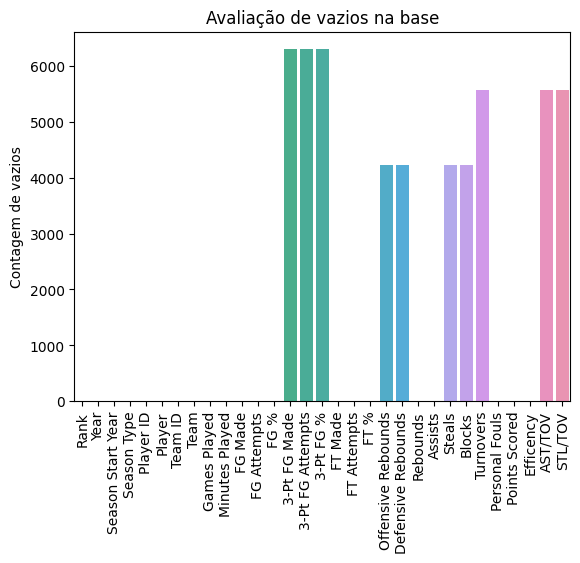
\includegraphics{imagens/1.png}

O DataFrame apresenta valores nulos em algumas colunas, como 3-Pt FG Made, 3-Pt FG Attempts, 3-Pt FG \%, Offensive Rebounds, Defensive Rebounds, Steals, Blocks, Turnovers, AST/TOV e STL/TOV. Esses valores nulos podem indicar a ausência de dados ou informações faltantes para algumas estatísticas específicas dos jogadores em determinadas temporadas.

Para manter a consistência e garantir a confiabilidade da análise, optou-se por filtrar o DataFrame, excluindo as temporadas anteriores a 1978. Dessa forma, as colunas mencionadas estarão preenchidas a partir desse ano, permitindo uma análise mais completa e precisa das estatísticas dos jogadores da NBA.

Essa decisão foi tomada para evitar distorções nos resultados devido à ausência de dados em períodos anteriores, garantindo que a análise seja baseada em informações mais completas e recentes.

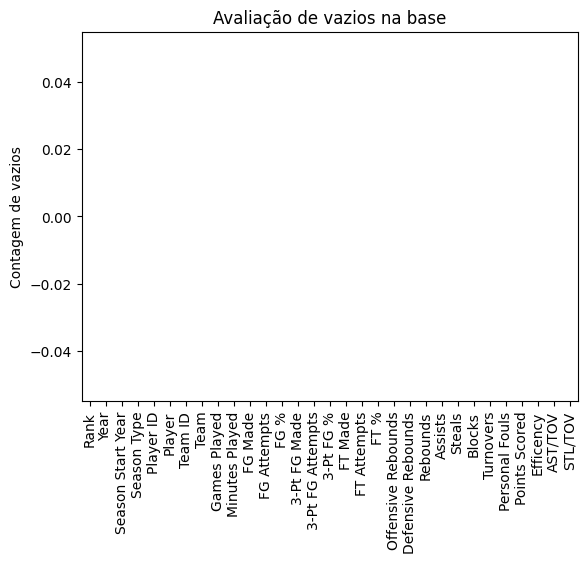
\includegraphics{imagens/2.png}

\hypertarget{o-que-define-um-jogador-bom}{%
\chapter{O que define um jogador bom?}\label{o-que-define-um-jogador-bom}}

Para simplificação, será utilizado o rank apresentado no dataset, que representa a ordenação dos jogadores de acordo com a pontuação por temporada.

Apesar desse rank não levar em consideração fatores defensivos, será feita uma avaliação para verificar se os maiores ``cestinhas'' também apresentam características defensivas acima da média.

Em um primeiro momento, será avaliado como as informações estatísticas de cada jogador por temporada variam e como estão relacionadas com o rank. Para isso, será utilizada a técnica do PCA para entender melhor esse comportamento.

Para definir o número ideal de componentes, avaliou-se a variância explicada por cada componente e utilizou-se a regra do cotovelo.

Observando o gráfico abaixo, pode-se notar que a partir da segunda componente, quase toda a variância é explicada. Portanto, duas componentes são suficientes para descrever os dados, além de facilitar a interpretação visual dos mesmos.

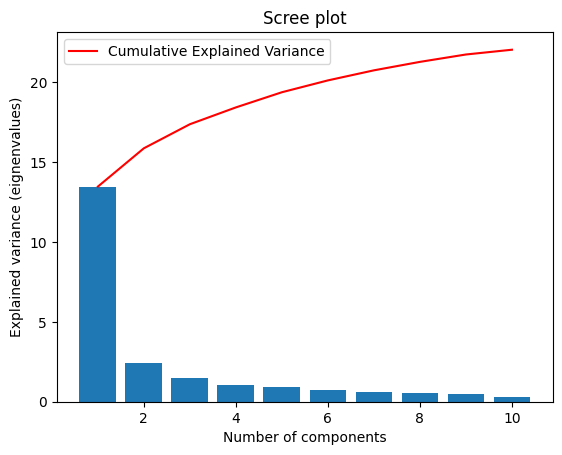
\includegraphics{imagens/3.png}

Na primeira análise do PCA, é possível observar que as variáveis são capazes de separar os jogadores com melhor ranking. Além disso, o ranking pode seguir três caminhos distintos, todos com a variável ``eficiência'' como a principal, mas com um foco maior em cestas de dois pontos, outro em cestas de três pontos, e por fim, um focado em rebotes e bloqueios. Esse último é especialmente relevante para jogadores nas posições de pivô e ala-pivô.

Além disso, nota-se a presença de muitas variáveis correlacionadas. Para análises futuras, serão removidas as variáveis com maior correlação e menor peso no PCA.

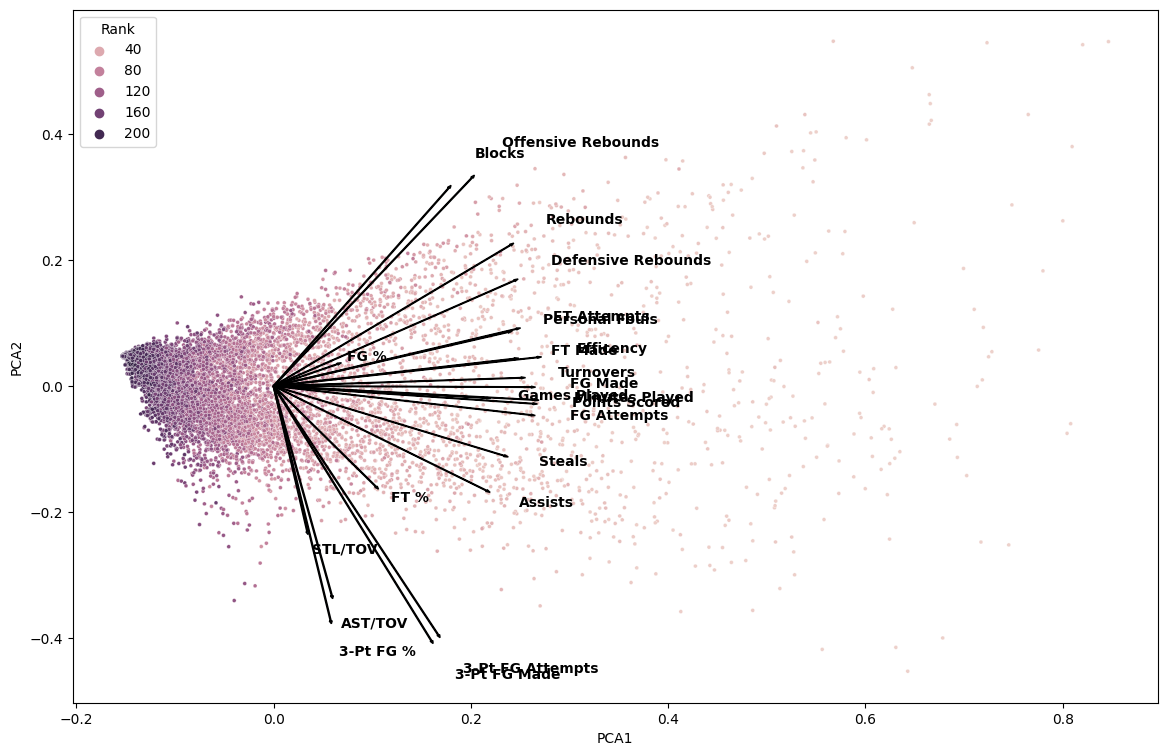
\includegraphics{imagens/4.png}

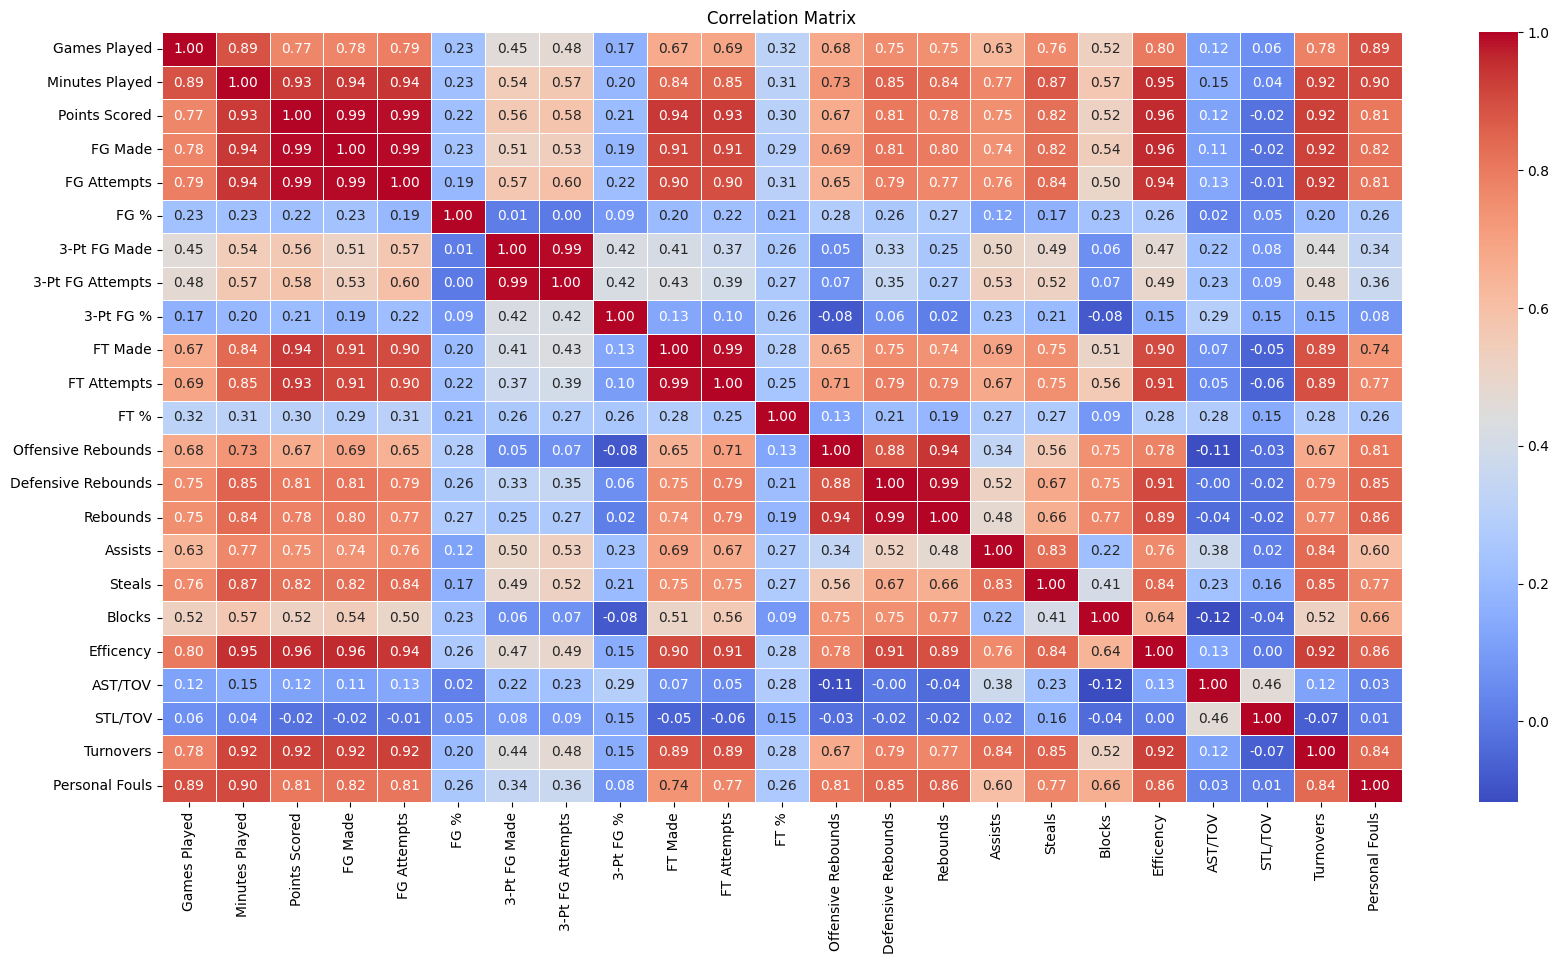
\includegraphics{imagens/5.png}

A matriz de correlação gerada apresenta os coeficientes de correlação entre diferentes variáveis. Os valores na matriz variam de -1 a 1 e indicam a força e direção do relacionamento entre as variáveis.

Aqui estão algumas observações com base na matriz de correlação:

\begin{itemize}
\item
  Há uma correlação positiva forte entre ``Games Played'' e várias outras variáveis, como ``Minutes Played'', ``FG Made'', ``FG Attempts'', ``FT Made'' e ``FT Attempts''. Isso faz sentido, uma vez que jogadores que disputam mais partidas tendem a acumular mais minutos de jogo e ter mais tentativas e acertos em arremessos de quadra e lances livres.
\item
  Existe uma correlação positiva forte entre ``Offensive Rebounds'' e ``Defensive Rebounds'', o que é esperado, já que ambos contribuem para o número total de rebotes.
\item
  Há uma correlação positiva forte entre ``Points Scored'' e várias outras variáveis, como ``FG Made'', ``FT Made'' e ``Minutes Played''. Isso indica que jogadores que marcam mais pontos também tendem a converter mais arremessos de quadra, lances livres e jogar por mais minutos.
\end{itemize}

Após a redução da dimensionalidade, é possível observar que as estatísticas ainda apresentam uma separação razoável na determinação do ranking dos jogadores. Além disso, os jogadores com os maiores rankings estão bem distantes do centróide.

Na figura abaixo, destacamos os cinco melhores jogadores de cada temporada, além de apresentar um exemplo para três jogadores: LeBron James, Shaquille O'Neal e Stephen Curry.

É interessante notar que, na avaliação desses três jogadores, Curry se destaca pelas cestas de três pontos, O'Neal pela presença no garrafão, com um elevado número de rebotes, e LeBron com uma das maiores eficiências já vistas na história da NBA.

Em resumo, para se definir um jogador bom, é necessário ter uma maior eficiência de maneira geral, sendo que essa eficiência pode variar de acordo com a posição e características dos jogadores. Por exemplo, um armador como Curry tem facilidade em fazer cestas de três pontos, enquanto um ala-pivô como LeBron possui características mais equilibradas e O'Neal, como pivô, se destaca pela presença no garrafão.

Por fim, mesmo que o ranking utilizado seja baseado na pontuação, nota-se que os jogadores mais bem ranqueados não se destacam apenas por essa característica.

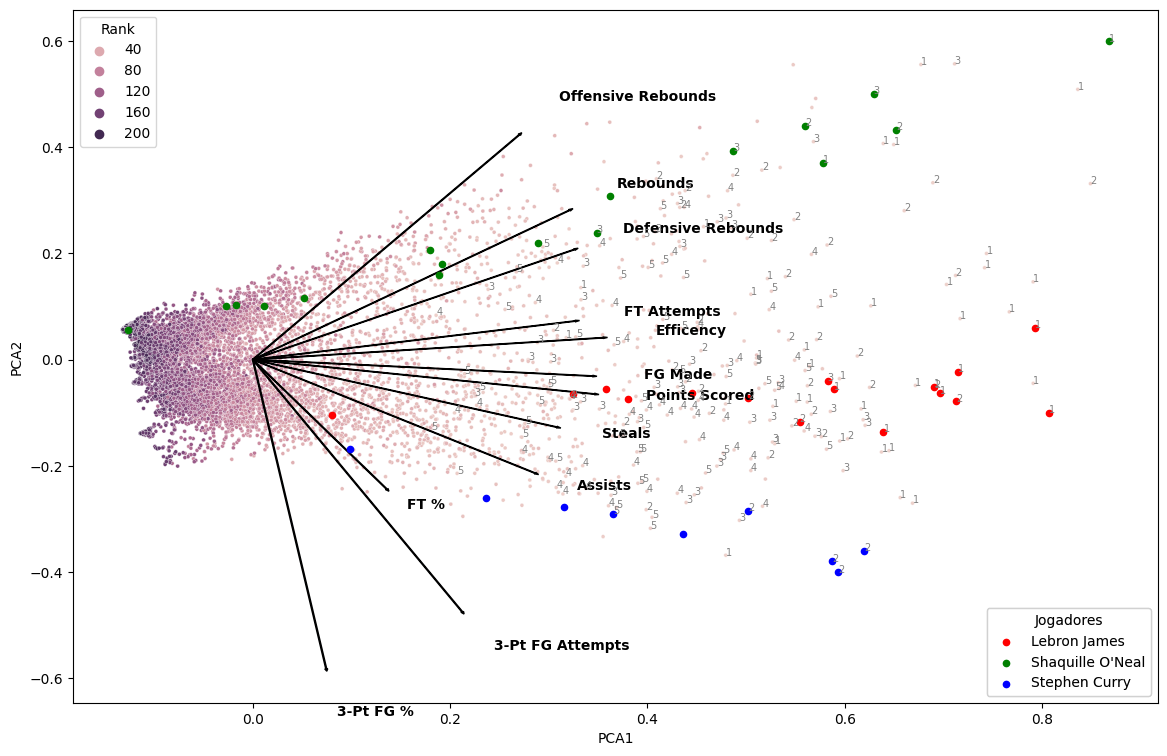
\includegraphics{imagens/6.png}

Para corroborar com a avaliação do PCA foi utilizada uma outra técnica a fim de verificar o poder de separação dos atributos da base, as Curvas de Andrews.
Elas são úteis porque permitem identificar quais variáveis têm um maior impacto na separação dos grupos, ajudando a entender a importância relativa de cada característica. Além disso, elas também podem ser usadas para detectar a presença de outliers ou padrões incomuns nos dados.

As Curvas de Andrews são construídas utilizando a série de Fourier para transformar as variáveis originais em uma combinação de funções seno e cosseno. A série de Fourier é uma representação matemática de uma função periódica como uma soma infinita de funções seno e cosseno com diferentes frequências.

A fórmula da série de Fourier utilizada para construir as Curvas de Andrews é a seguinte:

Fórmula de Fourier para Curvas de Andrews

\(\ f(x) = \frac{a_0}{2} + \sum_{n=1}^{\infty} \left( a_n \cos(nx) + b_n \sin(nx) \right)\)

Nesta fórmula, f(x) representa a função que descreve a curva de Andre para uma determinada variável. Os coeficientes a\_0, a\_n e b\_n são calculados com base nos dados originais e representam a amplitude e a fase das funções seno e cosseno em diferentes frequências.

Para cada variável do conjunto de dados, a série de Fourier é aplicada e os coeficientes a\_0, a\_n e b\_n são determinados. Em seguida, as séries de Fourier são somadas para criar a curva de Andrews para cada grupo no conjunto de dados.

Essa abordagem permite representar as variáveis em termos de frequências harmônicas, revelando padrões e relações entre elas. As Curvas de Andrews resultantes são plotadas em um gráfico para visualização e análise da separação entre os grupos.

A interpretação das Curvas de Andrews é baseada na análise da forma das curvas e na distância entre elas. Se as curvas de diferentes grupos estão próximas umas das outras, isso indica que as variáveis têm um poder de separação menor. Por outro lado, se as curvas estão bem separadas, isso sugere que as variáveis têm um alto poder de separação entre os grupos.

Quando é observada a curva, é possível notar que as variáveis selecionadas no PCA apresentam uma boa separação entre os grupos top 20,top 21-70, 71-150 e maior que 150, indicando que esses atributos separam bem não somente os melhores jogadores, como destacados no PCA, mas também entre jogadores menos bem ranqueados.

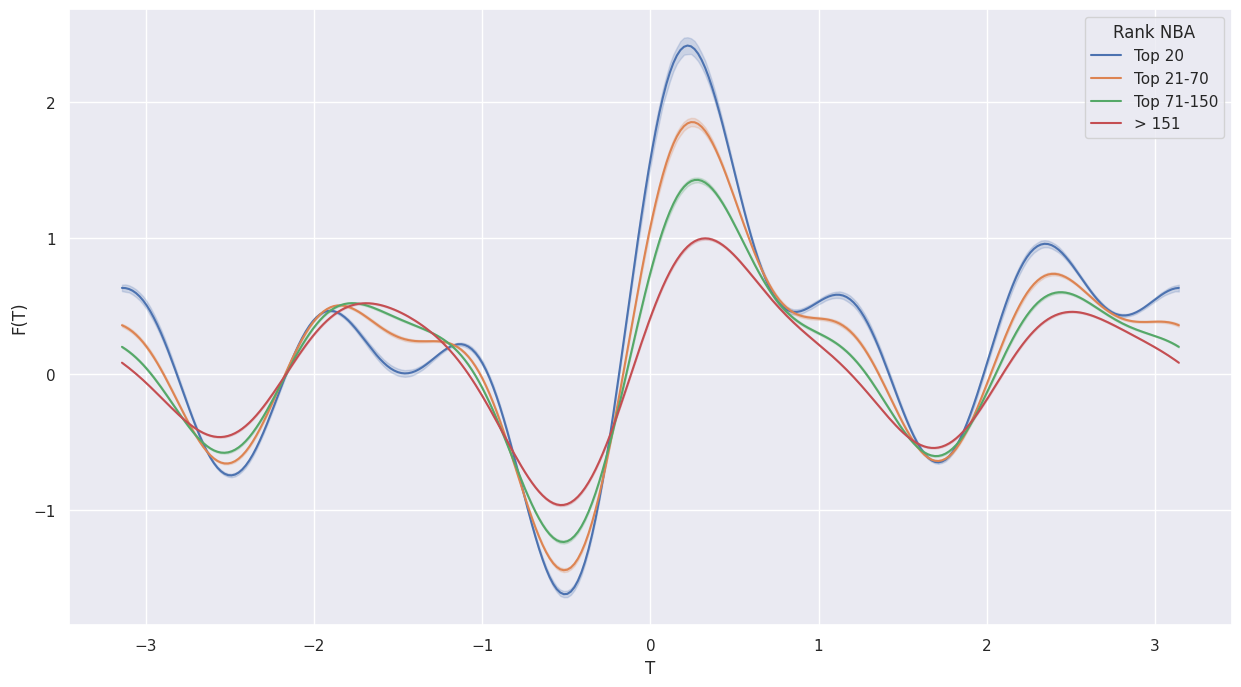
\includegraphics{imagens/7.png}

Por fim, a última avaliação dos jogadores foi realizada utilizando a técnica Radviz. Essa técnica é utilizada para visualizar dados multivariados. Consiste em um gráfico circular no qual os pontos de dados são dispostos ao redor de um círculo, sendo a posição de cada ponto determinada pelas suas variáveis. Cada variável é representada por um eixo radial, e a localização do ponto no gráfico indica a contribuição relativa de cada variável para o ponto de dados. Dessa forma, o Radviz permite identificar padrões e relacionamentos entre as variáveis de maneira intuitiva e compacta.

No caso da NBA, uma propriedade interessante é quando um jogador se destaca em vários atributos, ele ficará mais próximo do centro do círculo, enquanto jogadores que se destacam mais em um atributo específico tenderão a se afastar do centro.

Ao observar os top 20 jogadores, é possível notar que eles estão mais concentrados ao centro, indicando que seus atributos não se limitam a uma habilidade específica, mas apresentam resultados razoáveis em todos os atributos. Além disso, à medida que o ranking aumenta, os pontos se dispersam ao longo do círculo, indicando a presença de valores mais extremos.

Em resumo, de acordo com o Radviz, pode-se concluir que para ser considerado um bom jogador na NBA, não basta ser o principal pontuador, mas é necessário se destacar de maneira considerável em outros aspectos, como defesa, rebotes, variedade de arremessos e assistências.

\hypertarget{evoluuxe7uxe3o-do-jogo-ao-longo-dos-tempos-e-temporadas.}{%
\chapter{Evolução do jogo ao longo dos tempos e temporadas.}\label{evoluuxe7uxe3o-do-jogo-ao-longo-dos-tempos-e-temporadas.}}

Ao avaliar o Radviz aberto por ano e temporada (regular e playoffs), é possível chegar a algumas conclusões:

\begin{itemize}
\item
  Na década de 80/90, os arremessos de três pontos eram menos frequentes, e isso pode ser observado pela menor variação nos dados relacionados a essas estatísticas. As âncoras 3-pt FG\%, 3Pt FG Attempts e 3-pt FG Made não apresentam uma tendência clara. No entanto, nas décadas seguintes, há uma dispersão maior dos dados nessas âncoras, indicando uma maior importância e frequência dos arremessos de três pontos.
\item
  Os dados são mais dispersos na temporada regular do que nos playoffs, tornando mais difícil uma separação clara entre os jogadores mais bem ranqueados, especialmente nos top 150.
\item
  Nos playoffs, a dispersão dos dados é menor, permitindo uma melhor separação dos top 20 jogadores. É importante notar que alguns extremos podem ser encontrados entre os jogadores até o top 150, o que não ocorre na temporada regular.
\item
  Os top 20 jogadores da NBA, independentemente do ano ou da temporada, apresentam uma característica consistente: eles são constantes em todos os indicadores, sem apresentar extremos significativos.
\end{itemize}

Um exemplo disso é Stephen Curry, que é conhecido por seus arremessos de três pontos e sempre possui um alto ranking. No entanto, ele se mantém próximo ao centro no Radviz, indicando que ele também é bem avaliado em outros aspectos do jogo.

Essas observações mostram que a consistência e o desempenho equilibrado em várias estatísticas são características importantes para os jogadores de destaque na NBA.

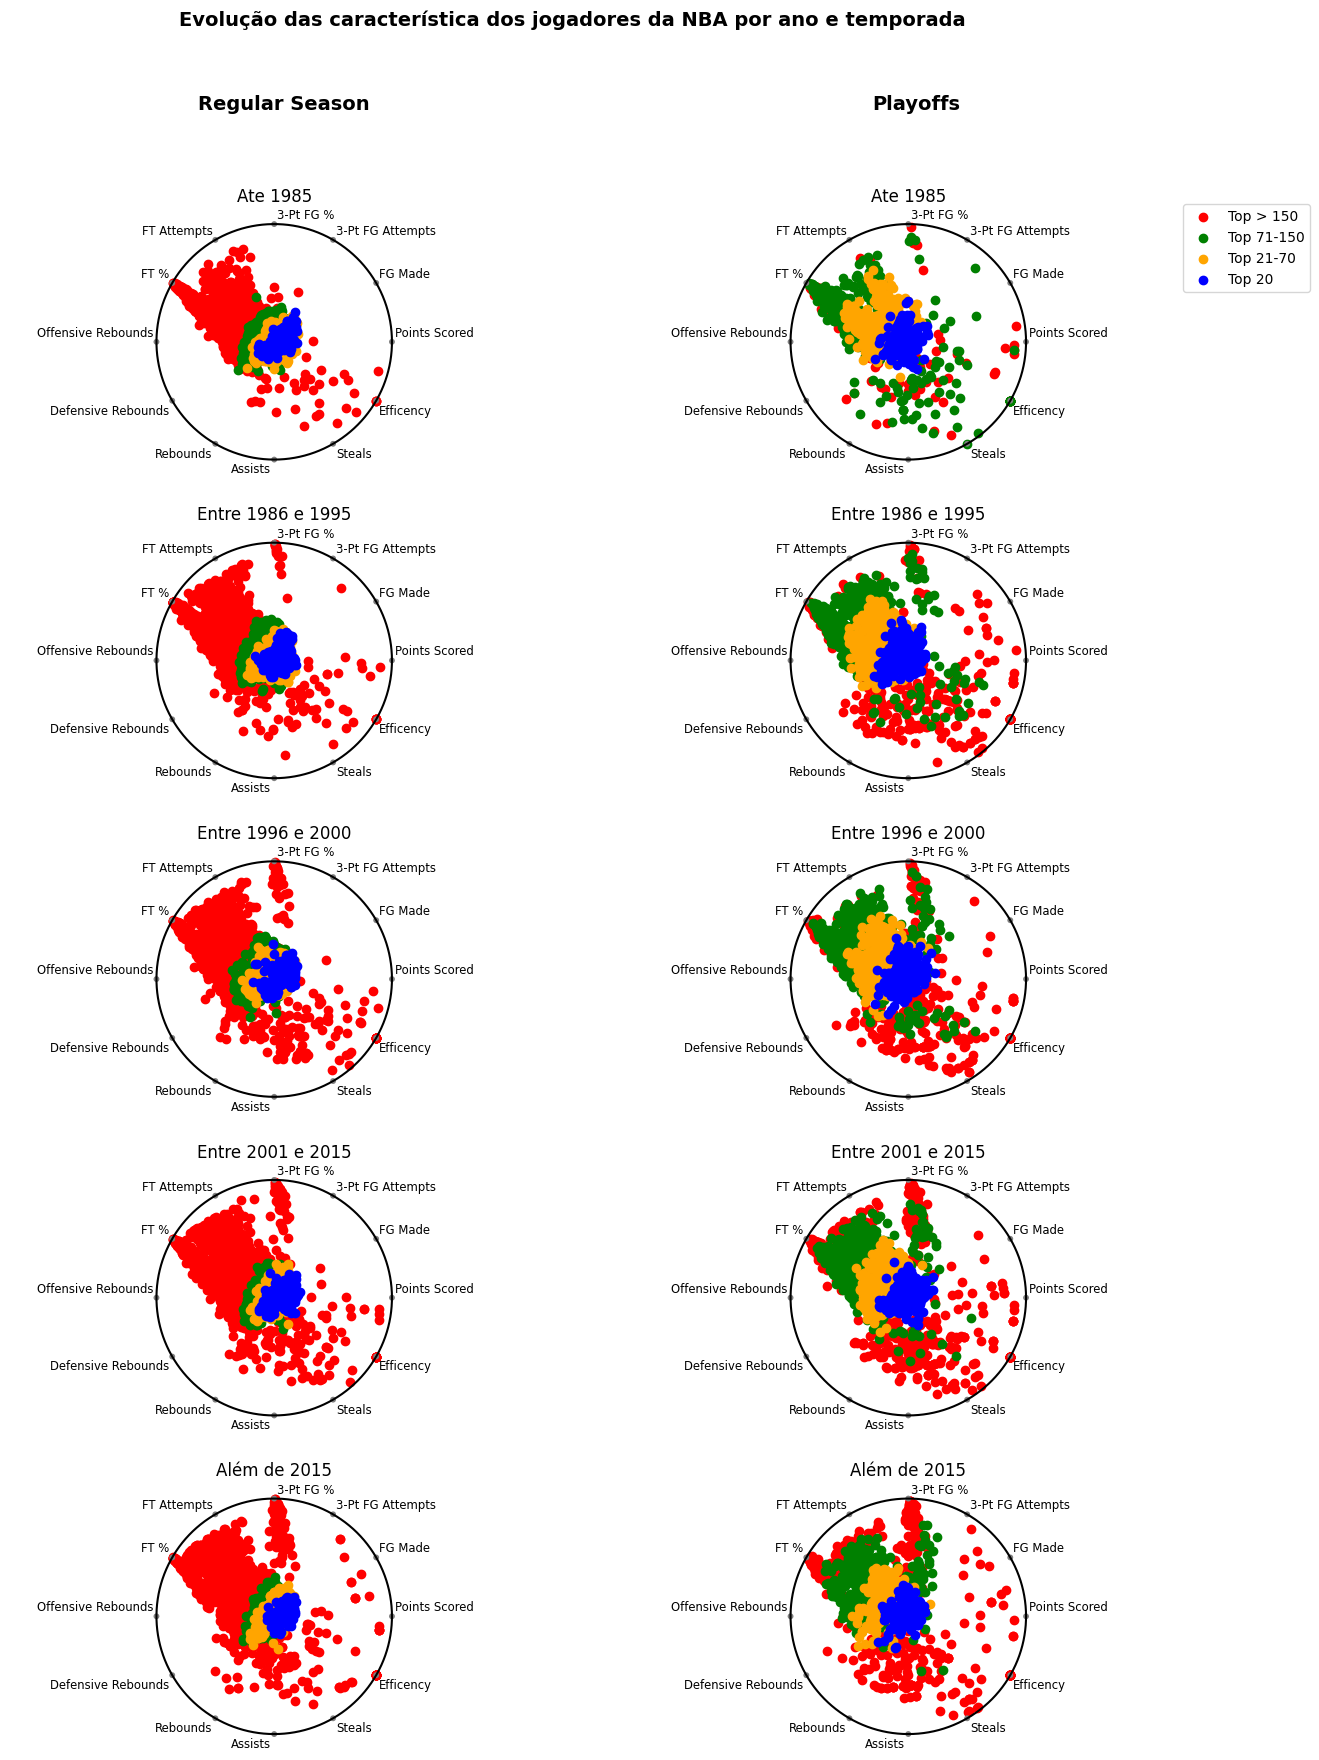
\includegraphics{imagens/14.png}

\hypertarget{entendimento-das-principais-estatuxedstica-do-jogo}{%
\chapter{Entendimento das principais estatística do jogo}\label{entendimento-das-principais-estatuxedstica-do-jogo}}

Ao avaliar o Radviz aberto por ano e temporada (regular e playoffs), é possível chegar a algumas conclusões:

\begin{itemize}
\item
  Na década de 80/90, os arremessos de três pontos eram menos frequentes, e isso pode ser observado pela menor variação nos dados relacionados a essas estatísticas. As âncoras 3-pt FG\%, 3Pt FG Attempts e 3-pt FG Made não apresentam uma tendência clara. No entanto, nas décadas seguintes, há uma dispersão maior dos dados nessas âncoras, indicando uma maior importância e frequência dos arremessos de três pontos.
\item
  Os dados são mais dispersos na temporada regular do que nos playoffs, tornando mais difícil uma separação clara entre os jogadores mais bem ranqueados, especialmente nos top 150.
\item
  Nos playoffs, a dispersão dos dados é menor, permitindo uma melhor separação dos top 20 jogadores. É importante notar que alguns extremos podem ser encontrados entre os jogadores até o top 150, o que não ocorre na temporada regular.
\item
  Os top 20 jogadores da NBA, independentemente do ano ou da temporada, apresentam uma característica consistente: eles são constantes em todos os indicadores, sem apresentar extremos significativos.
\end{itemize}

Um exemplo disso é Stephen Curry, que é conhecido por seus arremessos de três pontos e sempre possui um alto ranking. No entanto, ele se mantém próximo ao centro no Radviz, indicando que ele também é bem avaliado em outros aspectos do jogo.

Essas observações mostram que a consistência e o desempenho equilibrado em várias estatísticas são características importantes para os jogadores de destaque na NBA.

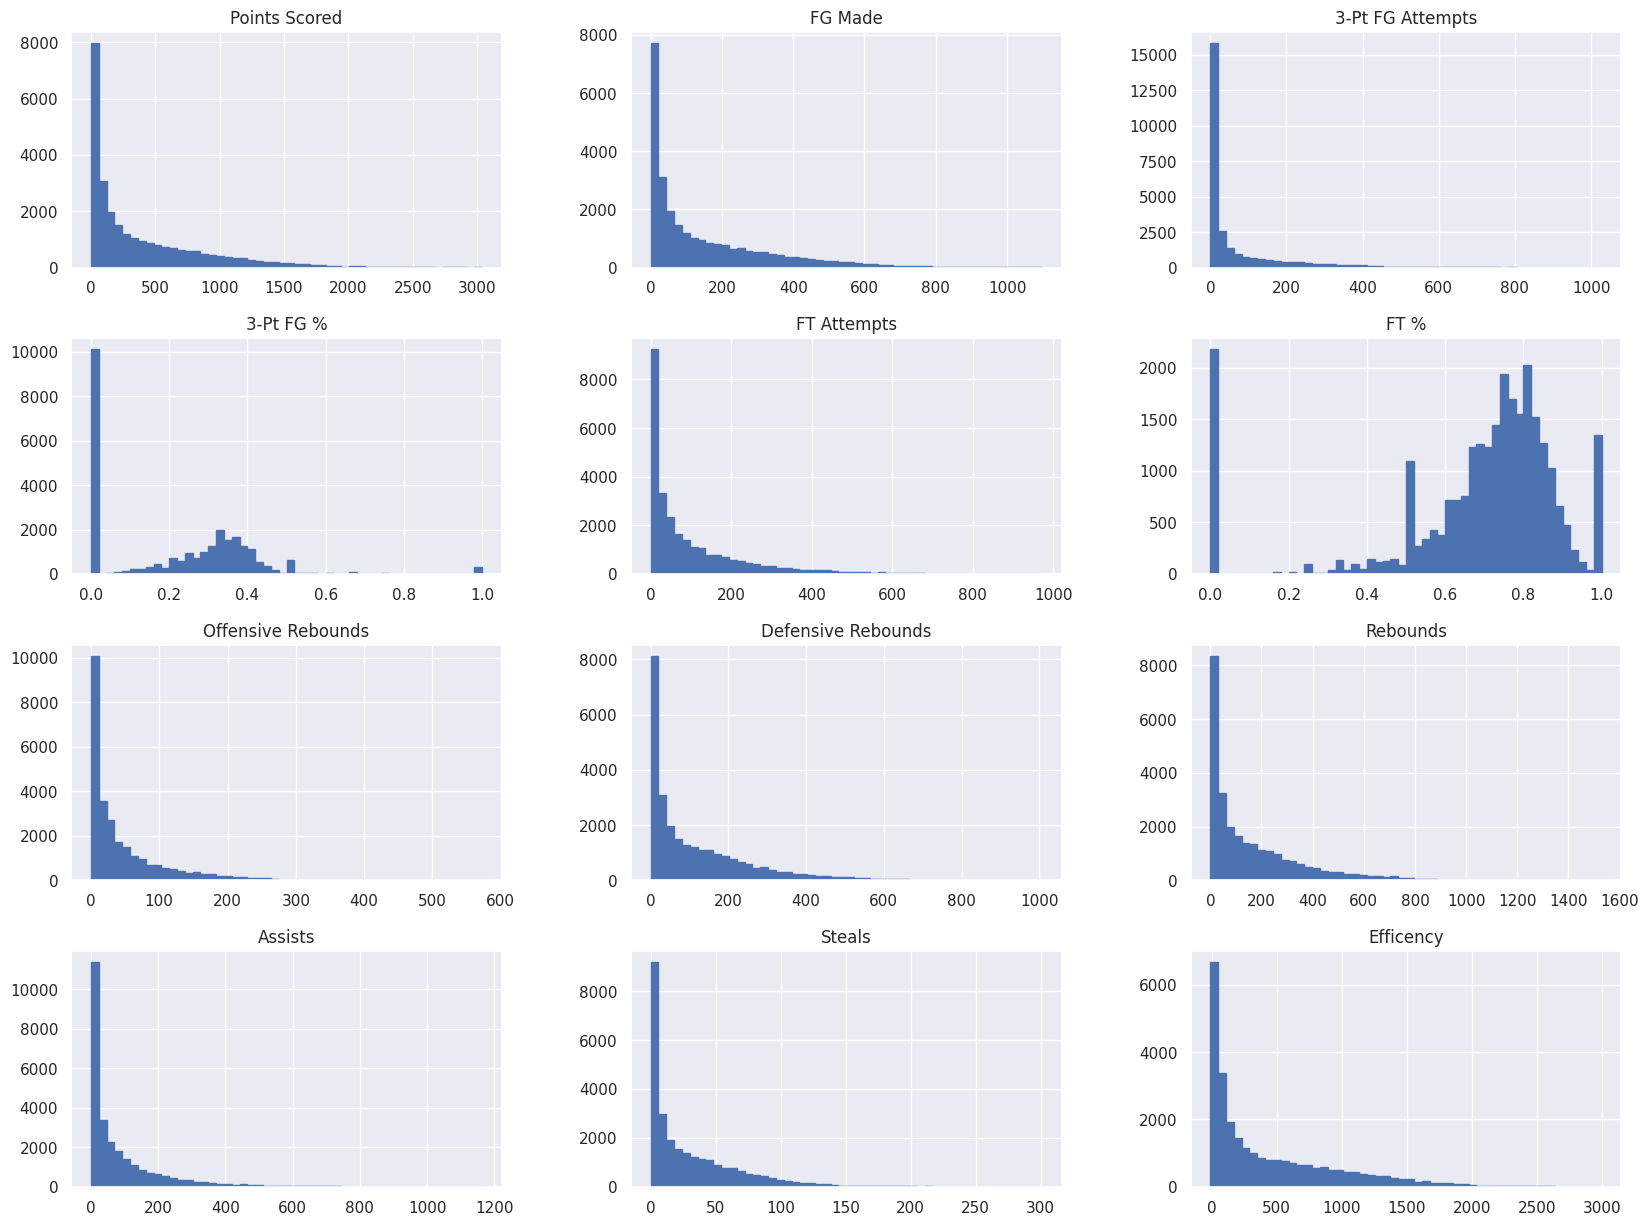
\includegraphics{imagens/15.png}

\textbf{Principais pontuadores de todos os tempos}

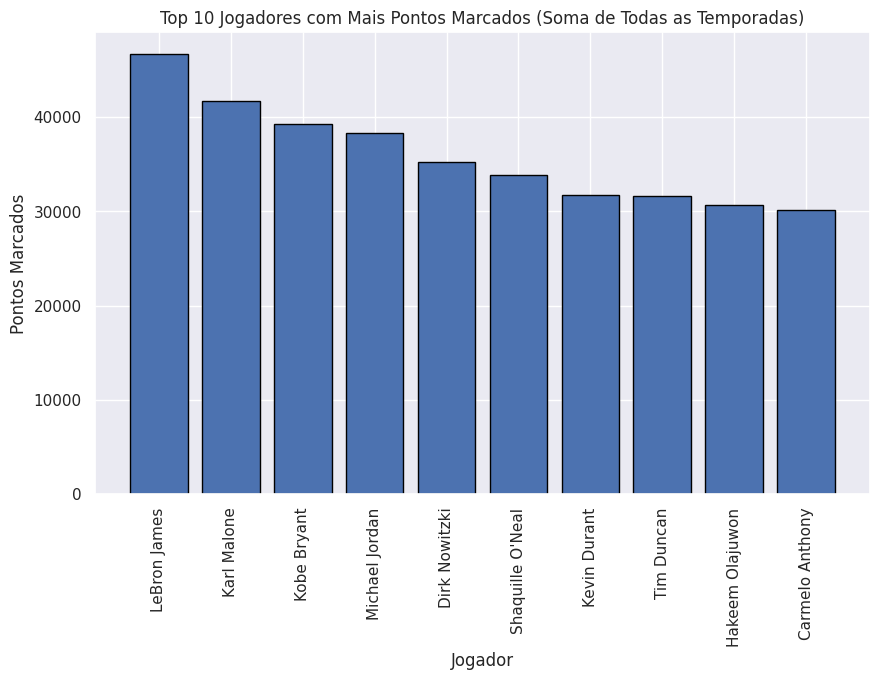
\includegraphics{imagens/16.png}

\textbf{Principais ``garçons'' de todos os tempos}

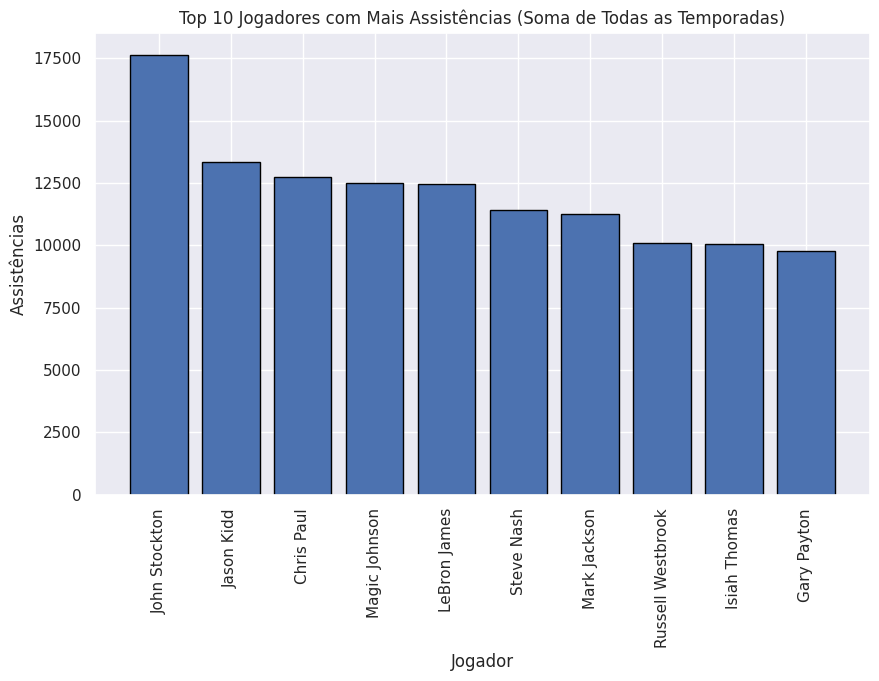
\includegraphics{imagens/17.png}

\textbf{Principais bloqueadores de todos os tempos}

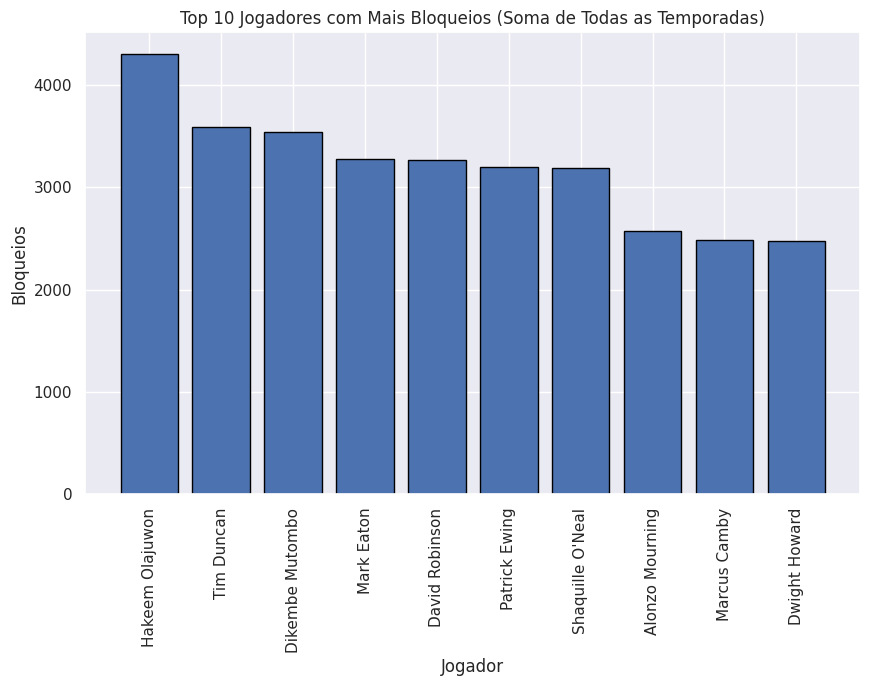
\includegraphics{imagens/18.png}

\textbf{Principais pontuadores dos três de todos os tempos}

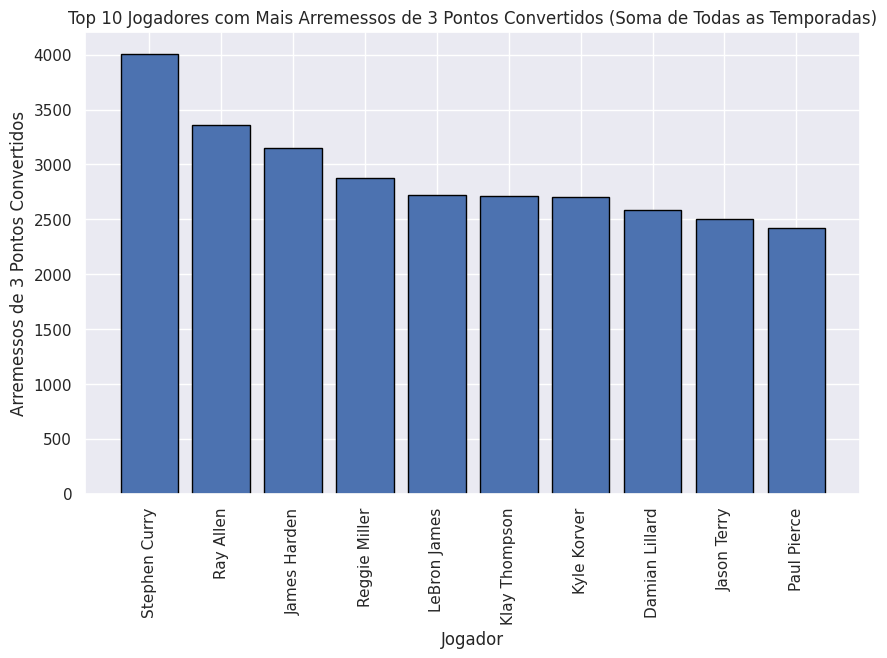
\includegraphics{imagens/19.png}

\hypertarget{o-que-define-um-time-bom}{%
\chapter{O que define um time bom?}\label{o-que-define-um-time-bom}}

\hypertarget{chernoff-faces}{%
\section{Chernoff Faces}\label{chernoff-faces}}

Últimos campeões e vices da NBA:

2013 - San Antonio Spurs \textbar{} Miami Heat

2014 - Golden State Warriors \textbar{} Cleveland Cavaliers

2015 - Cleveland Cavaliers \textbar{} Golden State Warriors

2016 - Golden State Warriors \textbar{} Cleveland Cavaliers

2017 - Golden State Warriors \textbar{} Cleveland Cavaliers

2018 - Toronto Raptors \textbar{} Golden State Warriors

2019 - Los Angeles Lakers \textbar{} Miami Heat

2020 - Milwaukee Bucks \textbar{} Phoenix Suns

2021 - Golden State Warriors \textbar{} Boston Celtics

2022 - Denver Nuggets \textbar{} Miami Heat

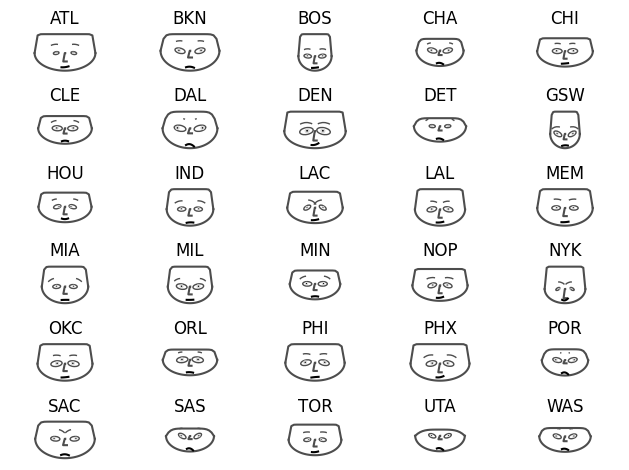
\includegraphics{imagens/20.png} 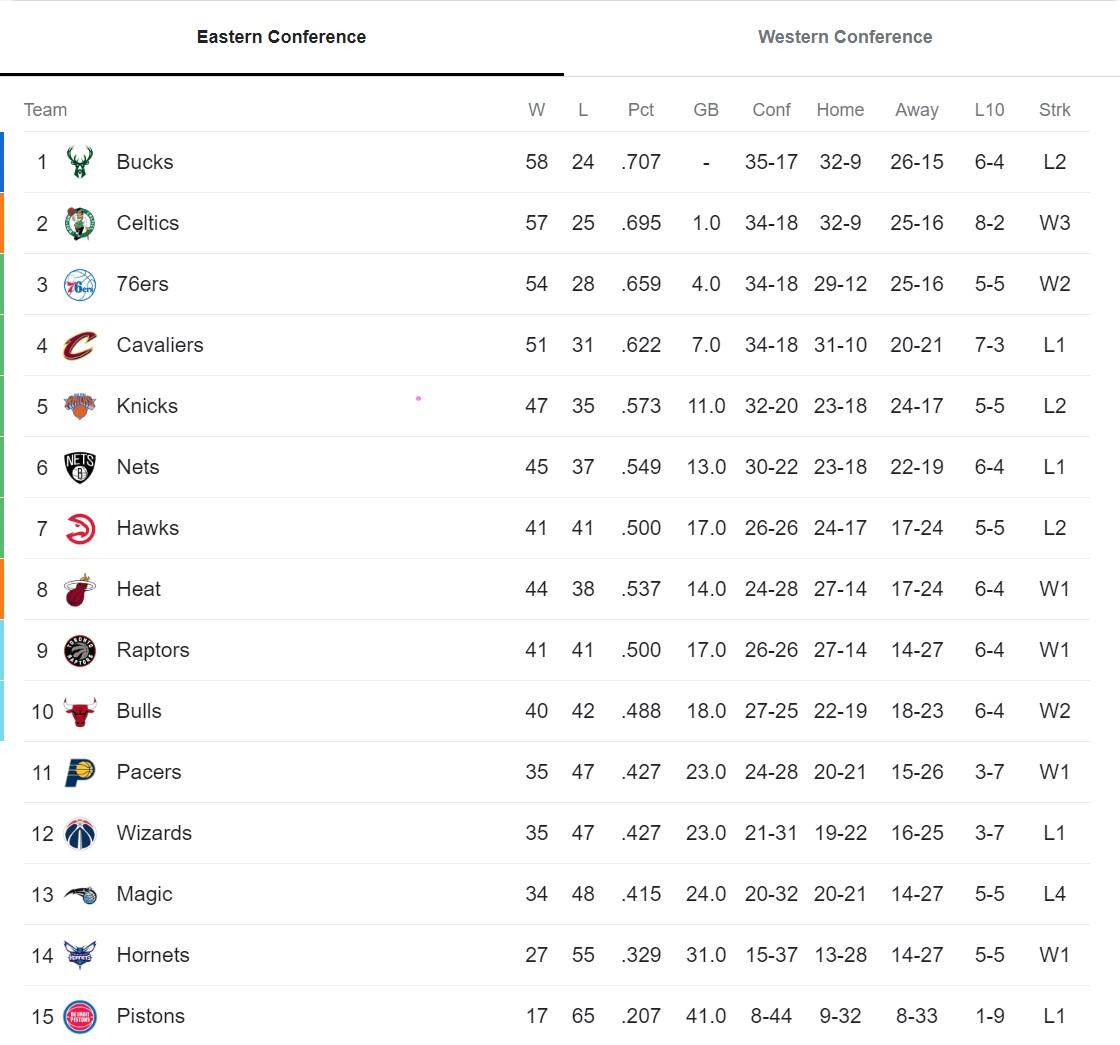
\includegraphics{imagens/21.jpeg} 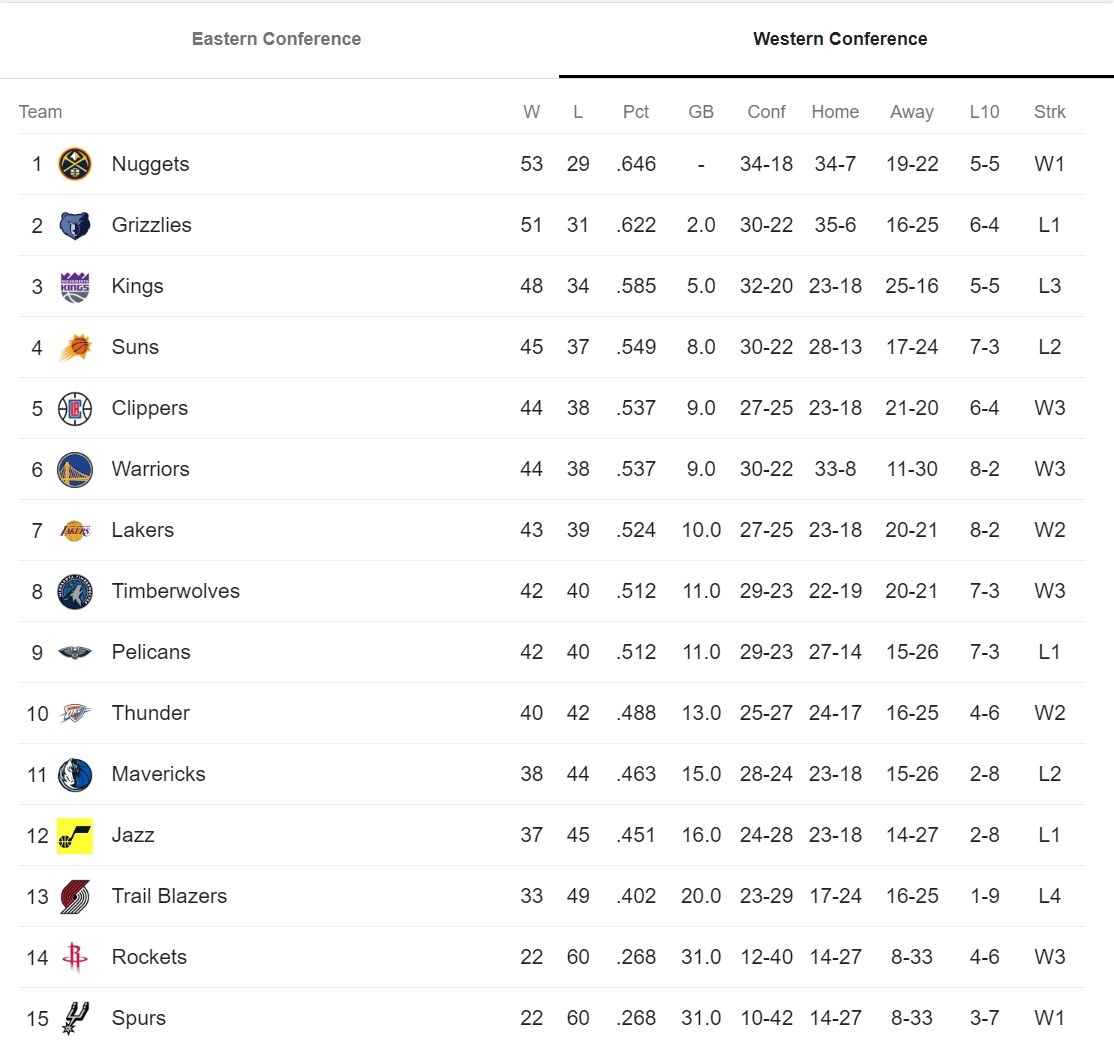
\includegraphics{imagens/22.jpeg} 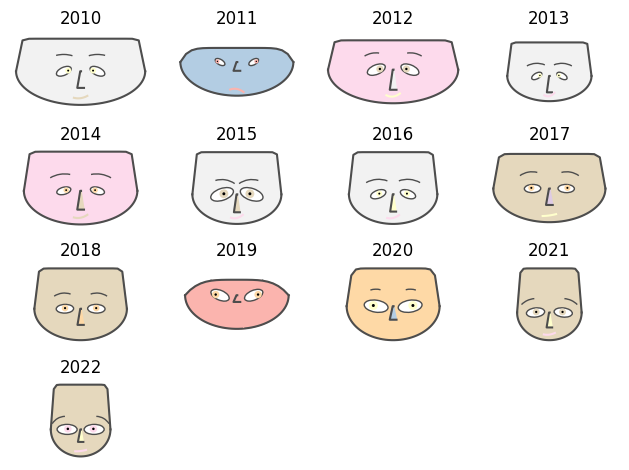
\includegraphics{imagens/23.png} Últimas posições na temporada regular do Golden State Warriors:

2010 - 3º

2011 - 4º

2012 - 2º

2013 - 2º

2014 - 1º

2015 - 1º

2016 - 1º

2017 - 1º

2018 - 1º

2019 - 5º

2020 - 4º

2021 - 2º

2022 - 4º

Concluindo, é possível observar tendencias de padrão e comportamento semelhantes em anos ou times que são parecidos, porém devido a natureza do gráfico e a falta de informação, principalmente para o ``usuário'' final, sobre os componentes representados por cada item (tamanho dos olhos, posição, inclinação da sobrancelha, etc.), não é possível fazer análises mais profundas.

Vemos como um gráfico de apoio para facilitar algumas visualizações ou fomentar questionamentos, por exemplo: os gráficos de 2015 e 2017 são significativamente diferentes, apesar do time ter sido campeão em ambas as temporadas. O desempenho nesses anos foi muito diferente? Ou então, os Pacers (IND) e os Wizards (WAS) tiveram o mesmo aproveitamento na temporada (0.427), porém seus gráficos são distintos. O que será que aconteceu? Sabemos que o resultado final de um jogo é apenas vitória ou derrota, porém a margem de pontos pode ser de 1 ou de 20, bem como a quantidade de arremesos, roubadas de bola, entre outros. Um time pode ter tido um desempenho comparável a times pior classificados e ter tido ``sorte'' de ganhar a quantidade suficiente de jogos, mesmo que por uma margem pequena e perder por muito, enquanto outro sempre tinha jogos parelhos, porém perdeu em mais ocasiões.

  \bibliography{book.bib,packages.bib}

\end{document}
